\documentclass[tikz,border=5pt]{standalone}
\usepackage{pgfplots}
\pgfplotsset{compat=1.18}

\definecolor{corba}{HTML}{365FB3}
\definecolor{punt}{HTML}{B91C1C}
\definecolor{guia}{HTML}{6B7280}

\begin{document}
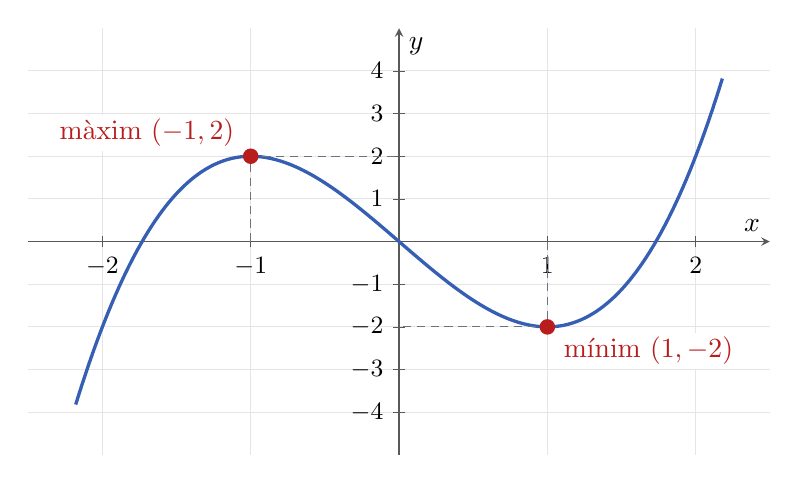
\begin{tikzpicture}
  \begin{axis}[
    width=11cm,
    height=7cm,
    axis lines=middle,
    xmin=-2.5,
    xmax=2.5,
    ymin=-5,
    ymax=5,
    xlabel={$x$},
    ylabel={$y$},
    xtick={-2,-1,1,2},
    ytick={-4,-3,-2,-1,1,2,3,4},
    grid=major,
    grid style={black!10},
    axis line style={black!65},
    tick style={black!65},
    tick label style={font=\small},
    clip=false,
  ]
    \addplot[corba, very thick, domain=-2.18:2.18, samples=180]
      {x^3-3*x};

    \draw[guia, densely dashed]
      (axis cs:-1,0) -- (axis cs:-1,2) -- (axis cs:0,2);
    \draw[guia, densely dashed]
      (axis cs:1,0) -- (axis cs:1,-2) -- (axis cs:0,-2);

    \addplot[only marks, mark=*, mark size=2.6pt, punt]
      coordinates {(-1,2) (1,-2)};

    \node[anchor=south east, text=punt, fill=white, inner sep=1.5pt]
      at (axis cs:-1.08,2.12) {màxim $(-1,2)$};
    \node[anchor=north west, text=punt, fill=white, inner sep=1.5pt]
      at (axis cs:1.08,-2.12) {mínim $(1,-2)$};
  \end{axis}
\end{tikzpicture}
\end{document}
